% !TEX root =  main.tex

%Description of \m\mEdhoc and main changes from last verified version

\subsection{About the protocol}

\vnote{Note for discussion with others: I find the macros for the protocol, method, and tool names distracting while reading through (the font changes too much, too often). The macro for \mEdhoc actually inserts a line break if you start a sentence with it, because of the \texttt{hbox} (I'm not sure why the hbox exists for what is a macro to be inserted in running text). I do need to start sentence with \mEdhoc many times though, so this is irritating. It is also the case that ProVerif needs to be written like so, and not capitalized entirely, so at least one of them is plain wrong! For now I've left in the macros, but I'd prefer that we fixed them to be regular capitalized text or, in the case of ProVerif, in camelcase as they should be.}

\vnote{Macros don't work right in section headers!}

\knote{We don't need to repeat the setting about why \mEdhoc{} is needed from
the introduction. This section should describe what \mEdhoc is.}
\vnote{I've removed the duplicate text. Let me know if it is okay now.}

Since \mEdhoc is a key exchange protocol, it is expected to provide perfect forward secrecy and identity protection. For providing application layer security, \mEdhoc makes use of \mCbor Object Signing and Encryption (\mCose)~\cite{rfc8152}. This works well in cases where transport layer security is not sufficient, or where multiple underlying protocols need to be accounted for. 

Agents participating in the \mEdhoc{} protocol can authenticate themselves to
peers using one out of three authentication methods -- digital signatures
(\mSig), challenge-response signatures based on static Diffie-Hellman keys
(\mStat) or pre-shared symmetric keys (\mPsk).
We will refer to these authentication methods simply as methods below.

Four combinations of the \mSig{} and \mStat{} authentication methods are possible,
while the \mPsk{} authentication method can only be run by an agent with another
agent also authenticating with a \mPsk.
We refer to these combinations also as methods, denoted \mSigSig, \mSigStat,
\mStatStat, \mStatSig{} and \mPskPsk.
Although the terminology is overloaded, it should be clear from the context
whether a single agent authentication method or a combined method is intended.

We describe each of these methods in detail later in this section.

%The communicating parties must agree on the method and cipher suite used for encryption as part of the first message. The parties exchange ephemeral public keys, compute the shared secret, and derive symmetric application keys from this secret.

The \mSig based methods of \mEdhoc are built on \mSigmaI, a variant of the \mSigma protocol which provides identity protection for the initiator, and  implements the \mSigmaI variant as Mac-then-Sign. The method involving static DH keys proceeds along the lines of \mOptls, with the agent creating a MAC and encrypting it using an algorithm for authenticated encryption with associated data (\mAead)~\cite{aead,rfc5116}. 

%\mEdhoc allows the initiator and responder to run different methods, combining \mSig and \mStat -- for example, the initiator might run a \mSig-based method, while the responder is running a \mStat-based method. This set of methods is not covered in previous versions of \mEdhoc, which only had a single \mSigma asymmetric key method (corresponding to the \mSigSig method shown in Section~\ref{sec:methods}). This allows one party to use a \mSigma style of authentication using signatures, while the other can use static DH keys. %In Figure~\ref{fig:edhocasym}, a template for all the asymmetric key methods of \mEdhoc is shown. 
%
%\begin{figure}[!h]
%\centering
%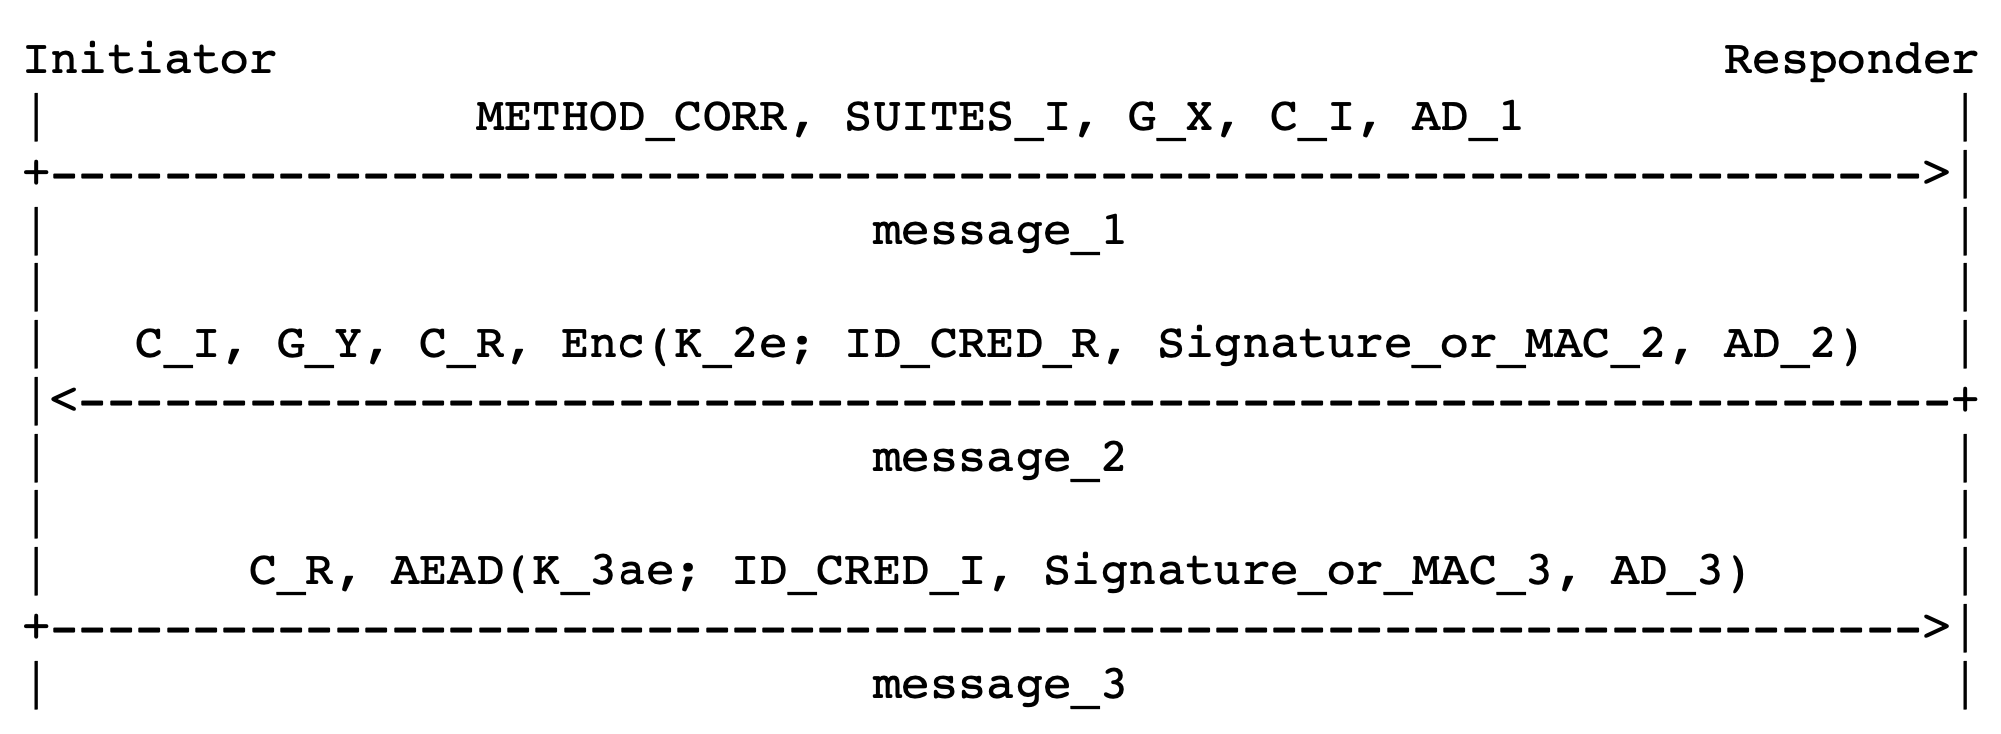
\includegraphics[scale=0.3]{Images/asym.png}
%\caption{A template for the asymmetric key methods of \mEdhoc}
%\label{fig:edhocasym}
%\end{figure}

%\subsection{Background, comparison with~\cite{DBLP:conf/secsr/BruniJPS18}}
%\knote{This section is again repetition from the introduction. Related work on
%    analyzing \mEdhoc should be in the related work section.
%    This section should describe \emph{what} \mEdhoc is IMHO.}
%The first version of \mEdhoc was proposed in March 2016 to a working group investigating lightweight authenticated key exchange protocols [\mcneed]. There has been a focus on formally verifying that the protocol satisfies the properties expected of it right from the beginning. 
%
%The 2018 work~\cite{DBLP:conf/secsr/BruniJPS18} by Bruni et al performed a formal verification of version 08 (\url{https://tools.ietf.org/html/draft-selander-ace-cose-ecdhe-08} \mcfix) of \mEdhoc. The protocol and properties are modelled and verified in the \mProverif tool. This version of the protocol belongs to the \mSigmaI family of protocols, and has two modes -- one with asymmetric keys, and one with pre-shared symmetric keys. Bruni et al showed that this version satisfies the requisite properties of identity protection, (perfect forward) secrecy of data, and strong authentication, upon completion of the protocol.
%
%\mEdhoc has undergone a lot of change since version 08, as will be described in the following sections, and the formal verification of the current version, therefore, is a worthwhile exercise.

\subsection{Comparison with \mOptls and \mNoise}
\subsubsection{\mOptls}
\mOptls~\cite{cryptoeprint:2015:978} is a key-exchange protocol developed upon which to base the design of the handshake protocol in \mTls 1.3. In its most basic form, \mOptls is composed of two messages between a client and a server, where the server has a secret static key $s$ and a DH key $g^{s}$. The client first sends to the server a message composed of a fresh nonce and some negotiated parameters, along with an ECDH key $g^{x}$. The server responds with a nonce of its own, some other negotiated parameters, an ECDH key $g^{y}$, and a MAC of all these values computed using a key derived from $g^{xs}$. At the end of the protocol, a session key is derived jointly from $g^{xs}$ and $g^{xy}$. The former ensures secrecy for as long as $s$ is secure, and the latter provides perfect forward secrecy in case $s$ is compromised.

It can be seen that in \mEdhoc, an \mStat role is very similar to being either the client or the server in an \mOptls execution. The \mStatStat method can be thought of as interleaving two \mOptls sessions. 
\knote{Do we need to draw some conclusions or just leave it with this
observations?}

\subsubsection{\mNoise}
For the \mStatStat method, since both parties are running a \mStat method, there is an obvious analogue in terms of the \mNoise framework~\cite{perrin2016noise}. \mNoise is a framework for a certain class of security protocols where all parties communicate using static DH keys whose structure also meets certain requirements of encryption etc. 

The closest \mNoise ``pattern'' to the \mStatStat method of \mEdhoc is the XX pattern. It can be seen that the first two messages in this method of \mEdhoc correspond perfectly to the first two messages of the XX pattern of the \mNoise framework. However, in the third message, the XX pattern requires the initiator to send their static key, followed by an encrypted payload using a key derived by a combination of the static key and an ephemeral key. In \mEdhoc, the static key and the payload are both encrypted in the same key, one depending on the key used for the second message, and on the static key of the initiator. This perhaps diverges from the XX pattern of \mNoise, and one can no longer directly claim that \mEdhoc enjoys the same properties as XX. As a potential direction for future work, we relegate the further investigation of this pattern of the \mNoise framework to see if there is any correspondence with the \mStatStat method.
\knote{Do we need to draw some conclusions or just leave it with this
observations?}
\vnote{For both OPTLS and NOISE, I don't see what conclusions there are to be drawn. If you can think of any, please add them.}

%\section{Methods and features of \mEdhoc}\label{sec:methods}
We are now ready to dive into the details of the various methods supported by \mEdhoc. Note that there are some fundamental components that are common to all the \mEdhoc methods. These components are the aforementioned \mCose objects, \mAead encryption~\cite{aead} , and, perhaps most importantly, the key derivation function (KDF) utilized to generate pseudorandom strings and encryption/decryption keys. We give a quick introduction to \mCose and \mAead for the sake of completeness, and we then flesh out the workings of the KDF in full detail, before moving on to discuss the \mEdhoc methods.
 
\subsection{Fundamental components of \mEdhoc}
\subsubsection{\mCose}
\knote{It is not clear to me from this description alone how these components relate
to \mEdhoc.}
\vnote{I hope the above paragraph before the section addresses that.}
\mCbor is a data format designed for small code size and small message size. The \mCbor Object Signing and Encryption (\mCose) protocol is used to create and process signatures, MACs, and encryption using \mCbor. 

A \mCose object contains bitstrings corresponding to (cryptographically) protected parameters, unprotected parameter, and the payload to be signed. This can be signed/encrypted/MACed, to obtain a resultant \mCose object containing the bitstring corresponding to the operation. The respective algorithms may also be fed some externally supplied data, which is carried along with the \mCose object, but is not part of it. \mEdhoc only uses the sxignature and encryption objects of \mCose. For encryptions, \mCose supports two different methods -- one where the recipient is not needed because the key is known implicitly, and one for all other cases. \mEdhoc only uses the former. 

A \mCoseEncrypt structure as used in \mEdhoc is a \mCbor array with a text field which contains the string ``Encrypt0'' to denote the use of the method with implicit recipient, a field for protected data, a field for externally supplied application data, and a field for ciphertext. All these fields store the corresponding bitstrings.

\subsubsection{\mAead}
Authenticated encryption with associated data, or \mAead, is an authenticated encryption operation. The algorithm takes in a key, a unique nonce, a plaintext, and some associated data, and outputs a ciphertext. The plaintext is both authenticated and encrypted, while the associated data is merely authenticated. The ciphertext is at least as long as the plaintext. When the plaintext is empty, the \mAead algorithm acts as a MAC on the associated data. 

The associated data is used to protect information that needs to be authenticated, but does not need to be kept confidential. It might be desirable to authenticate this information, although it must be left unencrypted to allow the system to function properly. Authentication is provided without copying the data into the plaintext.

\subsubsection{Key derivation function (KDF)}
\knote{This section (or another section) could describe the key hierarchy used
    by \mEdhoc, i.e., with session key material at the top (derived from
    $g^{xy}$ and possible static DH-keys, and from this, the PRKs are derived
    and from those the AEAD keys for each message and so on. Such a description
    and perhaps a figure, would make it easier to read the method sections
    later.
}
\vnote{I've restructured the text and added a couple of paragraphs. I don't think a figure will do very much, but I can try to add one if you want.}
One of the most important building blocks for \mEdhoc is the key derivation function based on \mHkdf~\cite{rfc5869}, which is used to generate the pseudorandom strings and keys for the encryption operations in the communicated messages. The three pseudorandom strings (\mPRKtwo, \mPRKthree, and \mPRKfour) are derived using the \mHkdfExtract function, while the keys  are generated using the \mHkdfExpand function. Both these functions are based on \mHmac~\cite{rfc2104}, which is a hashing system for message authentication.

%The \mHkdfExtract function is run with a salt and some input keying material (IKM) as input. It produces as output a pseudorandom string. For the \mPskPsk method alone, the salt is the key pre-shared between the initiator and the responder, while for the other methods, it is empty. The IKM for all \mEdhoc methods is the ECDH shared secret $g^{xy}$. 

There is a natural hierarchy obeyed by these pseudorandom strings. We start with the IKM $g^{xy}$. The pseudorandom string \mPRKtwo is generated by running the \mHkdfExtract function on the IKM (along with the pre-shared key as salt, in the case of the \mPskPsk method -- for the other methods, the salt is empty). For the \mPskPsk and \mSigSig methods, only one pseudorandom string is used (i.e. $\mPRKtwo = \mPRKthree = \mPRKfour$). For the three \mStat-based methods, however, we use at least two pseudorandom strings. \mPRKthree can either be equal to \mPRKtwo, or obtained by running \mHkdfExtract on \mPRKtwo and one other input. This other input is obtained by an exponentiation operation between a long term key and an ephemeral key -- the exact inputs to this operation depend on the role and the method being run, and will be described in detail later. Similarly, \mPRKfour can either be equal to \mPRKthree, or obtained by running \mHkdfExtract on \mPRKthree and one other such input. Thus, \mPRKtwo is used as input to the KDF to generate \mPRKthree, which is in turn used to generate \mPRKfour.

The keys used for the \mAead encryptions are augmented with the suffix `e', for encrypting the ciphertext, or with the suffix `m', for generating the MAC (MACs only feature in the methods involving asymmetric keys). There are four keys -- \mKtwom, \mKtwoe, \mKthreem, and \mKthreeae. The suffixes in the names of the pseudorandom strings indicate which keys they are used to generate. \mPRKtwo is used to generate the key \mKtwoe along with the appropriate transaction hash. \mPRKthree is used for the keys \mKtwom and \mKthreeae, while \mPRKfour is used to generate \mKthreem.

\begin{figure}[htp]
\centering
% !TEX root =  edhocProtocol.tex
% Start the picture
\begin{tikzpicture}[%
    >=latex,              % Nice arrows; your taste may be different
    start chain=going below,    % General flow is top-to-bottom
    node distance=10mm and 60mm, % Global setup of box spacing
    every join/.style={norm},   % Default linetype for connecting boxes
    ]
% ------------------------------------------------- 
% A few box styles 
% <on chain> *and* <on grid> reduce the need for manual relative
% positioning of nodes
\tikzset{
terminput/.style={rounded corners, text width=6em},
term/.style={rounded corners},
  base/.style={draw, thick, on chain, on grid, align=center, minimum height=6ex},
  prk/.style={base, draw=Red3, fill=Red3!25, rectangle, text width=4em},
  %hkdfext/.style={base, draw=Green3, fill=Green3!25, isosceles triangle, isosceles triangle apex angle=60, anchor=base, shape border rotate=-90, text width=6em},
  hkdfext/.style={base, draw=Green3, fill=Green3!25, rectangle, text width=8em},
  %hkdfexp/.style={base, draw=orange, fill=orange!50, isosceles triangle, isosceles triangle apex angle=60, anchor=base, shape border rotate=-90, text width=6em},
  hkdfexp/.style={base, draw=orange, fill=orange!50, rectangle, text width=8em},
  keyb/.style={base, draw=Blue3, fill=Blue3!25, rectangle, text width=4em},
  % -------------------------------------------------
  norm/.style={->, draw, Blue3},
}
% -------------------------------------------------
% Start by placing the nodes
\node [prk] (p0) {$g^{xy}$};
\node [hkdfext, join] (h1) {\mHkdfExtract};
\node [prk, join] (p2) {\mPRKtwo};
\node [hkdfext, join] (h3) {\mHkdfExtract};
\node [prk, join] (p3) {\mPRKthree};
\node [hkdfext, join] (h5) {\mHkdfExtract};
\node [prk, join] (p4) {\mPRKfour};

\node [hkdfexp, shape border rotate=180, left= 3cm of p4] (h6) {\mHkdfExpand};
\node [keyb, join, left=3cm of h6] (k3) {\mKthreem};

\node [hkdfexp, shape border rotate=180, left= 3cm of p3] (h4) {\mHkdfExpand};
\node [keyb, join, left=3cm of h4] (k2) {\mKtwom};

\node [hkdfexp, shape border rotate=180, left= 3cm of p2] (h2) {\mHkdfExpand};
\node [keyb, join, left=3cm of h2] (k1) {\mKtwoe};

\node [hkdfexp, shape border rotate=180, below= 1cm of h4] (h8) {\mHkdfExpand};
\node [keyb, below=1cm of k2] (k2b) {\mKthreeae};
%\node [draw=none, fill=none, below=0.5cm of h4] (dummy) {};

\draw [->, norm] (p3.south) -- ++(0,-0.58) -- (h8);
\draw [->, norm] (h8) -- (k2b);
\draw [->, norm] (p2) -- (h2); 
\draw [->, norm] (p3) -- (h4); 
\draw [->, norm] (p4) -- (h6);
%\node [term, fill=Green3!25, below = -1.3cm of h1] (h1name) {\mHkdfExtract};
%\node [term, left = 1cm of h1name] (u1) {H1};
%\draw [->, dotted, shorten >=1mm] (u1) -- (h1name);
\node [terminput, right = 1cm of h1] (u1) {Initial salt};
\draw [->, dotted, shorten >=1mm] (u1) -- (h1);

%\node [term, fill=Green3!25, below = -1.3cm of h3] (h3name) {\mHkdfExtract};
%\node [term, left = 1cm of h3name] (u2) {H2};
%\draw [->, dotted, shorten >=1mm] (u2) -- (h3name);
\node [terminput, right = 1cm of h3] (u2) {Additional input};
\draw [->, dotted, shorten >=1mm] (u2) -- (h3);

\node [terminput, right = 1cm of h5] (u3) {Additional input};
\draw [->, dotted, shorten >=1mm] (u3) -- (h5);


%\node [term, fill=orange!50, below = -0.9cm of h2] (h2name) {\mHkdfExpand};
%\node [term, above = 1cm of h2name] (u3) {H3};
%\draw [->, dotted, shorten >=1mm] (u3) -- (h2);
\node [term, above = 1cm of h2] (u4) {\mTHtwo};
\draw [->, dotted, shorten >=1mm] (u4) -- (h2);

%\node [term, fill=orange!50, below = -0.9cm of h4] (h4name) {\mHkdfExpand};
%\node [term, above = 1cm of h4name] (u5) {H5};
%\draw [->, dotted, shorten >=1mm] (u5) -- (h4);
\node [term, above = 1cm of h4] (u5) {\mTHtwo};
\draw [->, dotted, shorten >=1mm] (u5) -- (h4);

\node [term, above = 0.7cm of h6] (u6) {\mTHthree};
\draw [->, dotted, shorten >=1mm] (u6) -- (h6);
\draw [->, dotted, shorten >=1mm] (u6) -- (h8);
%
% ------------------------------------------------- 
% 
%\path (h2.east) to node [near start, yshift=1em] {$n$} (c3); 
%  \draw [o->,lccong] (h2.east) -- (p8);
%\path (p3.east) to node [yshift=-1em] {$k \leq 0$} (c4r); 
%  \draw [o->,lcnorm] (p3.east) -- (p9);
% -------------------------------------------------
% 
%\path (h1.east) to node [near start, yshift=1em] {$n$} (c1); 
%  \draw [o->,lcfree] (h1.east) -- (c1) |- (p4);
%\path (h3.east) -| node [very near start, yshift=1em] {$n$} (c1); 
%  \draw [o->,lcfree] (h3.east) -| (c1);
%\path (p3.west) to node [yshift=-1em] {$k>0$} (c4); 
%  \draw [*->,lcnorm] (p3.west) -- (c4) |- (p3);
%\path (h4.east) -| node [very near start, yshift=1em] {$n$} (c6); 
%  \draw [o->,lcfree] (h4.east) -| (c6); 
%\path (h5.east) to node [near start, yshift=1em] {$n$} (c6); 
%  \draw [o->,lcfree] (h5.east) -| (c7); 
%\path (p4.east) to node [yshift=-1em] {$k \leq 0$} (c7); 
%  \draw [o->,lcfree] (p4.east) -- (c7)  |- (p9);
%\path (p4.west) to node [yshift=-1em] {$k>0$} (c5); 
%  \draw [*->,lcfree] (p4.west) -- (c5) |- (p5);
% -------------------------------------------------
% A last flourish which breaks all the rules
%\draw [->,MediumPurple4, dotted, thick, shorten >=1mm]
%  (p9.south) -- ++(5mm,-3mm)  -- ++(27mm,0) 
%  |- node [black, near end, yshift=0.75em, it]
%    {(When message + resources available)} (p0);
% -------------------------------------------------
\end{tikzpicture}
% =================================================

\caption{A diagram to illustrate the KDF key hierarchy}
\label{fig:kdfdiagram}
\end{figure}

In order to generate these keys, the \mHkdfExpand function is used. This is run with a pseudorandom string, an info string, and the length of the output keying material (OKM) as input. The pseudorandom string is generated using \mHkdfExtract as above. The info string contains details of the \mAead encryption algorithm used, length of the OKM, and the transaction hash as used for the specific method (a detailed discussion follows, for each method). In case the length $l$ of the OKM is shorter than that of the transaction hash, the OKM is obtained by taking the first $l$ bits of the result of running \mHmac on the pseudorandom string, and a concatenation of 0x01 and the info strings. The KDF hierarchy is illustrated in Figure~\ref{fig:kdfdiagram}.



We now discuss each of the \mEdhoc methods in detail over the next few sections.

\subsection{\mPskPsk method}
In this method, the initiator and responder are assumed to have a pre-shared key (\mPsk) which is secret to them, and can be retrieved by the responder using a public part of the first message (\mIDPsk). This method corresponds to the symmetric key method of \mEdhoc v08. 

In the first message, the initiator sends a message consisting of the method name, the cipher suites ranked in order of preference, the initiator's ephemeral key (\mGx), their connection identifier (\mCi), the \mIDPsk identifier, and (optional) auxiliary data (\mADone). The responder, upon receipt of this message, must verify that the selected cipher suite is supported,  and pass \mADone to the security application which needs it. If any verification step fails, the initiator sends an \mEdhoc error message back, and the protocol aborts.

The second message, sent by the responder, is composed of \mCi, the responder's ephemeral key \mGy, their connection identifier \mCr, and a \mCose object. This contains as external data the transaction hash of the first message (\mTHtwo), along with an \mAead encryption of the (optional) auxiliary data \mADtwo. The key used for this (\mKtwoae) is derived using the \mEdhoc key derivation function with \mTHtwo and the pseudorandom string \mPRKtwo as input, while the associated data for the \mAead encryption is constructed by concatenating a constant string, plaintext \mhplain, and \mTHtwo. Recall that the PRKs in this method are constructed by running \mHkdfExtract using \mPsk as salt. 

The initiator, upon receipt of this message, sends back \mCr, followed by a \mCose object containing an \mAead encryption of auxiliary data \mADthree, along with the hash of \mTHtwo and the encryption object received from the responder (which is referred to as \mTHthree) as external data. There is no protected data for this encryption. As earlier, the key used (\mKthreeae) is derived by supplying \mTHthree and \mPRKthree (which is the same as \mPRKtwo, for this method) as input to the KDF, and the associated data obtained by concatenating the constant string, plaintext \mhplain, and \mTHthree. An abstract description is shown in Figure~\ref{fig:edhocpsk}.

\begin{figure}[!h]
\centering
%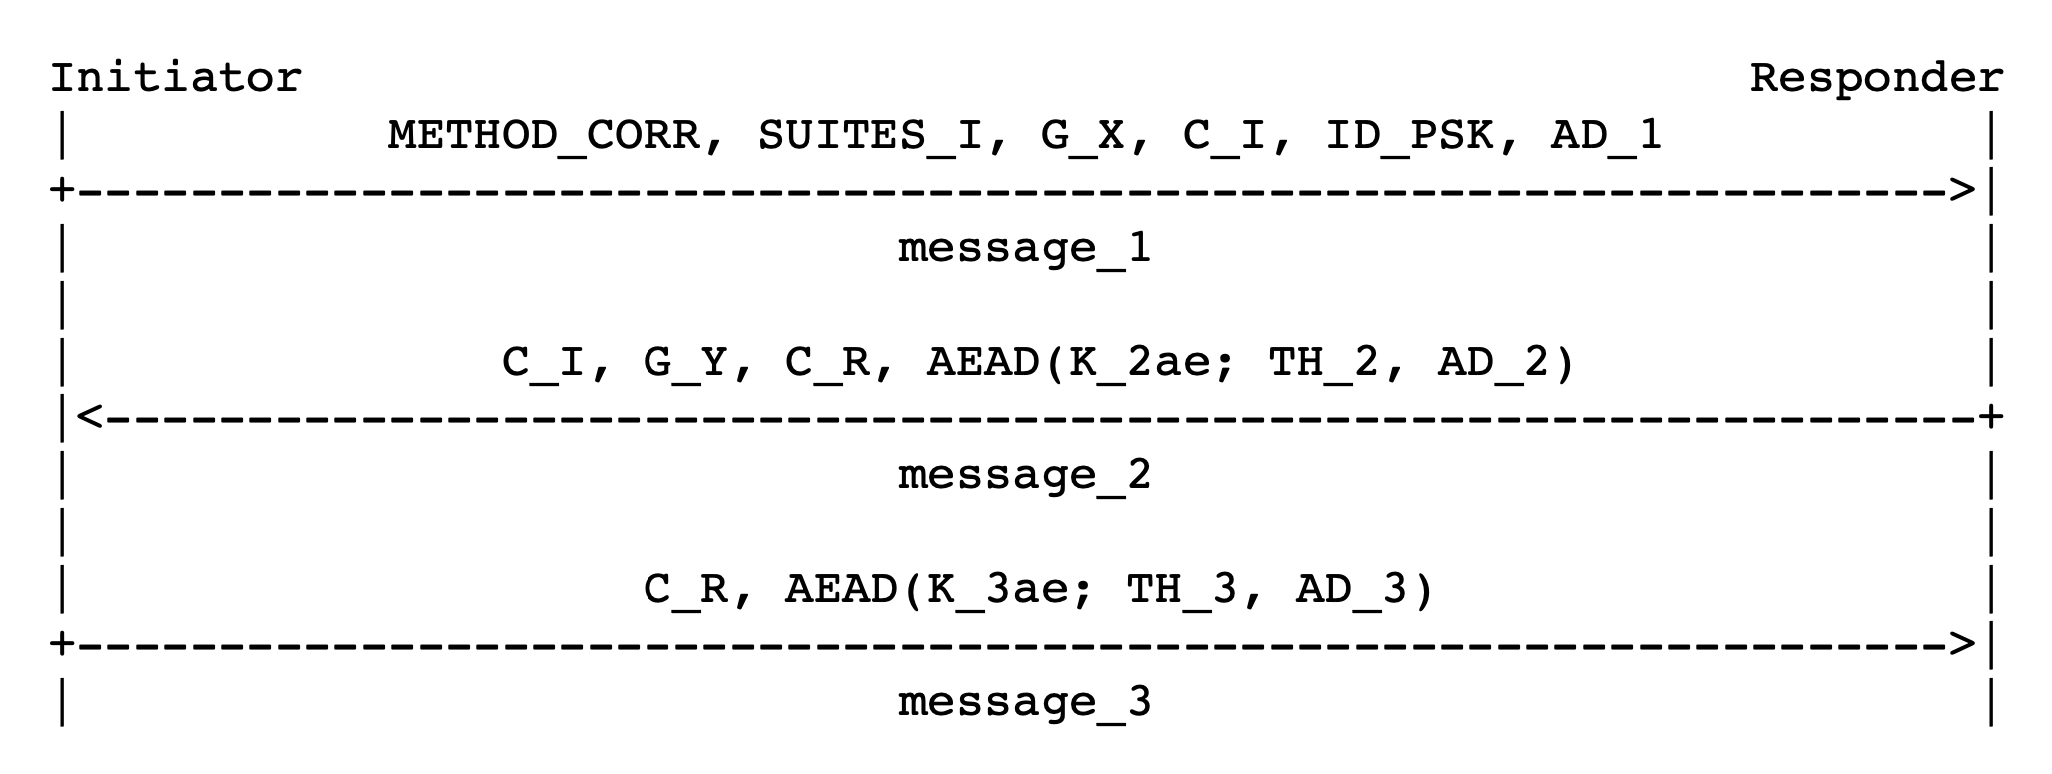
\includegraphics[scale=0.3]{Images/psk.png}
\scalebox{.7}{
\tikzset{>=latex, every msg/.style={draw=thick}, every node/.style={fill=white,text=black}}
\begin{tikzpicture}
    \node (ini) at (0, 0) {Initiator};
    \draw [very thick] (0, -0.5) -- (0,-11);
    \draw [very thick] (11.5, -0.5) -- (11.5,-11);
    \node[below of=ini,fill=white,text=black] () {Knows $g,\ \mPsk,\ \mIDPsk,\ \mADone,\ \mADthree$};
    \node (res) at (11.5,0) {Responder};
    \node[below of=res] () {Knows $g,\ \mPsk,\ \mIDPsk,\ \mADtwo$};
    \action{4em}{ini}{Generates \mMethod,\ \mSuites,\ \mCi,\ $x$\\$\mGx = g^{x}$};
    \msg{8em}{ini}{res}{\mMsgone: \mMethod, \mSuites, \mGx, \mCi, \mIDPsk, \mADone};
    \action{9em}{res}{$
      \begin{array}{c}
        \text{Generates } \mCr,\ $y$\\
        \mGy = g^{y}\\
        \mTHtwo = \mHash(\mMsgone, g^{y})\\
        \mPRKtwo = \mHkdfExtract(\mPsk, g^{xy}) \\
        \mKtwoae = \mHkdfExpand(\mPRKtwo, \mTHtwo)
      \end{array}$};
    \msg{18em}{res}{ini}{\mMsgtwo: \mCi, \mGy, \mCr, $\overbrace{\mAead(\mKtwoae; \mTHtwo, \mADtwo)}^{\mCipher}$};
    \action{19em}{ini}{$
      \begin{array}{c}
       \mTHtwo = \mHash(\mMsgone, \mGy)\\
       \mPRKtwo = \mHkdfExtract(\mPsk, g^{xy}) \\
        \mKtwoae = \mHkdf(\mPRKtwo, \mTHtwo)\\
        \mTHthree = \mHash(\mTHtwo, \mCipher)\\
        \mPRKthree = \mPRKtwo \\
        \mKthreeae = \mHkdfExpand(\mPRKthree, \mTHthree)
      \end{array}$};
    
    \msg{28em}{ini}{res}{\mMsgthree: \mCr, \mAead(\mKthreeae; \mTHthree; \mADthree)};
    \action{29em}{res}{$
    \begin{array}{c}
    	\mPRKthree = \mPRKtwo \\
        \mKthreeae = \mHkdfExpand(\mPRKthree, \mTHthree)
    \end{array}$};
    \draw [line width=2mm] (-2,-11) -- (2,-11);
    \draw [line width=2mm] (9.5,-11) -- (13.5,-11);
    \end{tikzpicture}}
\caption{The \mPskPsk method of \mEdhoc. $\mAead(x; y; z)$ is used to denote AEAD encryption where $x$ is the key, $y$ is a tuple of the protected and external data, and $z$ is the plaintext.}
\label{fig:edhocpsk}
\end{figure}


\subsection{\mStat-based methods}
\mEdhoc allows for three \mStat-based methods -- two where only one participant has a static Diffie-Hellman key (while the other uses signatures), and one where both do. 

In the first message, the initiator includes an identifier for the method, a preference-ordered list of cipher suites, their ephemeral key \mGx, their connection identifier \mCi, and some optional plaintext \mADone. This message is common to all the four methods below involving asymmetric keys. 

The responder, upon receipt, verifies the cipher suites, passes any \mADone to the application that needs it, and proceeds to construct and send the second message. This message contains (not necessarily all of) \mCi, \mGy, \mCr, and an encrypted term. The initiator, upon getting this message, sends out a message containing an encrypted term. Depending on the methods being run by the initiator and responder, the exact contents of these messages may vary. We will now describe each of these methods and the second and third messages therein in detail.

\subsubsection{\mSigStat}
The initiator runs a \mSigma-based method, with signatures, while the responder operates with a static Diffie-Hellman key and MACs. Both the initiator and the responder generate ephemeral secrets $x$ and $y$, and also have their respective long term public-private authentication keypairs. The public authentication keys have identifiers for retrieval as well.

The responder generates an ephemeral secret $y$, and an identifier \mCr. Then, it generates the pseudorandom strings. \mPRKtwo is obtained, as mentioned earlier, by running the KDF algorithm on the empty salt and the shared secret $g^{xy}$. Then, \mPRKthree is obtained by running the KDF algorithm on \mPRKtwo and \mGrx -- this is the result of raising the initiator's ECDH ephemeral public key \mGx to the responder's private authentication key \mLtkr. These pseudorandom strings will be used to generate encryption keys for this message.

The encrypted term for the second message is constructed as follows. First, we build the \mCose object that is the inner MAC, since the responder runs \mStat. The protected part of this object is an identifier for retrieving the responder's public authentication key, namely \mIdcredr. The externally supplied data is the transaction hash \mTHtwo (obtained by hashing the first message and \mGy),  the responder's public authentication key \mCredr, and (optional) auxiliary data \mADtwo. The plaintext is empty. The key used for the encryption \mKtwom is the output of the KDF on being fed as input the pseudorandom string \mPRKthree and \mTHtwo. The resulting encrypted object is now referred to as the ciphertext \mMactwo. 

For the outer encryption object, we consider the plaintext formed by concatenating the bitstrings corresponding to the identifier for \mCredr, \mMactwo, and \mADtwo (if any). The ciphertext is obtained by performing an \mXor operation on this plaintext with the key \mKtwoe, which is obtained by using the KDF on \mPRKtwo and the transaction hash \mTHtwo. The responder therefore sends to the initiator \mGy, \mCr, and this ciphertext as the second message.

First the initiator generates \mPRKtwo, using the same arguments to the KDF as the responder did above. For \mPRKthree, however, the initiator sends to the KDF \mPRKtwo and \mGrx -- this \mGrx is obtained by exponentiating \mCredr, the public authentication key of the responder, to the initiator's ephemeral secret $x$. Note that this will be used to generate a key to decrypt the inner \mMactwo sent by the responder, and therefore is asymmetric in nature to the \mGrx used by the responder above. \mPRKfour is set equal to \mPRKthree. 

It then sends the third message, consisting of \mCr, and an encrypted object. Here, again, we first build the inner \mCose object. This process is analogous to that employed by the responder for the second message. The \mCose object has as protected data an identifier for retrieving the initiator's public authentication key \mCredi. The externally supplied data is the transaction hash \mTHthree of the second message and \mTHtwo,  the initator's public authentication key \mCredi, and (optional) auxiliary data \mADthree. The key used is \mKthreem, obtained by inputing the pseudorandom string \mPRKthree and \mTHthree. The resulting encrypted object is now referred to as the ciphertext \mMacthree. 

Since the initiator is running \mSig, this \mCose object needs to be signed. To the signing algorithm, the initiator sends as protected data the identifier for retrieving \mCredi, as external data the concatenation of \mTHthree, \mCredi, and any \mADthree, and the payload \mMacthree. This is signed using the private authentication key of the initiator.  

We now construct the encryption for the third message, by passing to an \mAead encryption algorithm a \mCose object with no protected data, external data \mTHthree, and a plaintext obtained by concatenating the identifier for retrieving \mCredi, the signed object described above, and \mADthree. The key used for encryption is \mKthreeae, obtained by running the KDF on the pseudorandom string \mPRKthree and \mTHtwo. Thus, the message sent by the initiator to the responder in the third step is \mCr accompanied by this encrypted object. This method is illustrated in Figure~\ref{fig:edhocsigstat}.

\begin{figure}[!h]
\centering
%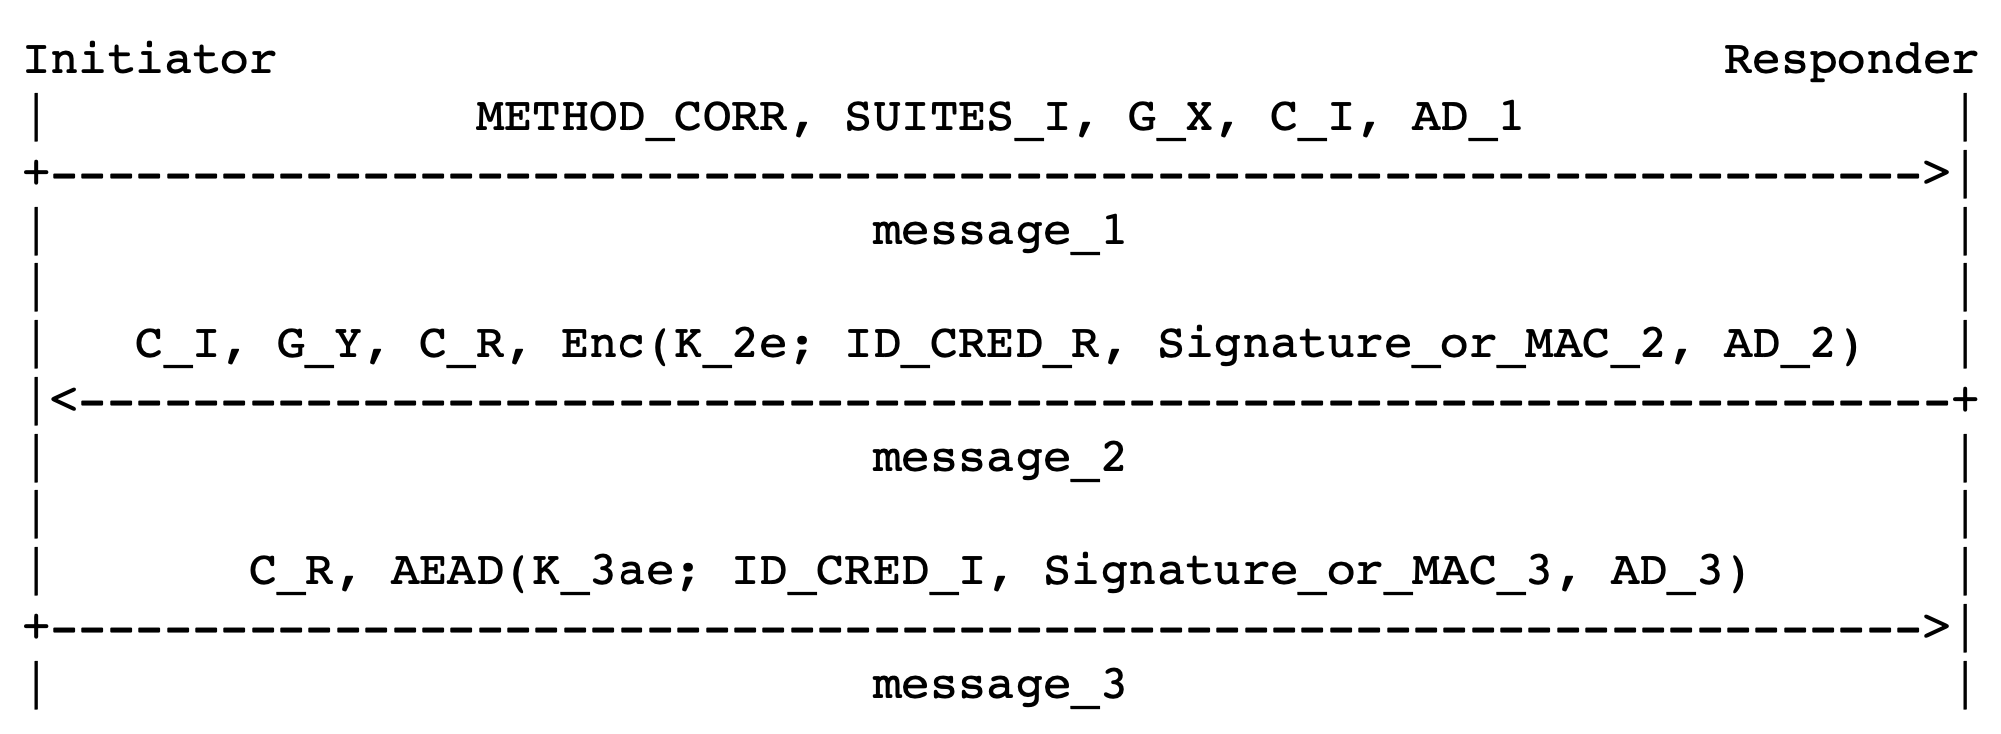
\includegraphics[scale=0.3]{Images/asym.png}
\scalebox{.7}{
\tikzset{>=latex, every msg/.style={draw=thick}, every node/.style={fill=white,text=black}}
\begin{tikzpicture}
    \node (ini) at (0, 0) {Initiator};
    \draw [very thick] (0, -0.5) -- (0,-15);
    \draw [very thick] (9, -0.5) -- (9,-15);
    \node[below of=ini,fill=white,text=black] {$
    \begin{array}{c}
    \text{Knows}\ $g$,\ \mCredi,\ \mLtki,\ \mIdcredi,\\
    \mCredr,\ \mIdcredr, \mADone,\ \mADthree
    \end{array}
    $};
    \node (res) at (9,0) {Responder};
    \node[below of=res] {$
    \begin{array}{c}
    \text{Knows}\ $g$,\ \mCredr,\ \mLtkr, \ \mIdcredr,\\
    \mCredi,\ \mIdcredi, \mADtwo
    \end{array}$};
    \action{5em}{ini}{Generates \mMethod,\ \mSuites,\ \mCi,\ $x$\\$\mGx = g^{x}$};
    \msg{10em}{ini}{res}{\mMsgone: \mMethod, \mSuites, \mGx, \mCi, \mADone};
    \action{11em}{res}{$
      \begin{array}{c}
        \text{Generates } \mCr,\ $y$\\
        \mGy = g^{y}\\
        \mTHtwo = \mHash(\mMsgone, \langle \mCi, \mGy, \mCr \rangle)\\
        \mPRKtwo = \mHkdfExtract(\textrm{``\phantom{}''}, g^{xy}) \\
        \mGrx = \mGx^{\mLtkr} \\
        \mPRKthree = \mHkdfExtract(\mPRKtwo, \mGrx) \\
        \mKtwom = \mHkdfExpand(\mPRKthree, \mTHtwo) \\
        \mMactwo = \mAead(\mKtwom; \langle \mIdcredr, \mTHtwo, \mCredr, \mADtwo \rangle; \textrm{``\phantom{}''}) \\
        \mKtwoe = \mHkdfExpand(\mPRKtwo, \mTHtwo)
      \end{array}$};
    \msg{26em}{res}{ini}{\mMsgtwo: \mCi, \mGy, \mCr, $\overbrace{\mKtwoe\ \mXor\ \langle \mIdcredr, \mMactwo, \mADtwo \rangle}^{\mCipher}$};
    \action{27em}{ini}{$
      \begin{array}{c}
        %\mTHtwo = \mHash(\mMsgone, \langle \mCi, \mGy, \mCr \rangle) \
        \mPRKtwo = \mHkdfExtract(\textrm{``\phantom{}''}, g^{xy}) \\
        %\mKtwoe = \mHkdfExpand(\mPRKtwo,\mTHtwo)\\
        \mGrx = \mCredr^{x} \\
        \mPRKfour = \mPRKthree = \mHkdfExtract(\mPRKtwo, \mGrx) \\
        %\mKtwom = \mHkdfExpand(\mPRKthree, \mTHtwo) \\
        \mKthreeae = \mHkdfExpand(\mPRKthree, \mTHtwo) \\
        \mTHthree = \mHash(\mTHtwo, \mCipher, \mCr)\\
        \mKthreem = \mHkdfExpand(\mPRKfour, \mTHthree) \\
        \mMacthree = \mAead(\mKthreem; \langle \mIdcredi, \mTHthree, \mCredi, \mADthree \rangle; \textrm{``\phantom{}''}) \\
        \mSigthree = \mSign(\mLtki; \langle \mIdcredi, \mTHthree, \mCredi, \mADthree \rangle, \mMacthree \rangle)
      \end{array}$};
    \msg{39em}{ini}{res}{$\mMsgthree: \mCr, \mAead(\mKthreeae; \mTHthree; \langle \mIdcredi, \mSigthree, \mADthree \rangle$)};
    \action{40em}{res}{$
    \begin{array}{c}
        \mTHthree = \mHash(\mTHtwo, \mCipher, \mCr)\\
        \mKthreem = \mHkdfExpand(\mPRKthree, \mTHthree) \\
        \mKthreeae = \mHkdfExpand(\mPRKthree, \mTHthree)
    \end{array}$};
    \draw [line width=2mm] (-2,-15) -- (2,-15);
    \draw [line width=2mm] (7,-15) -- (11,-15);
    \end{tikzpicture}}
\caption{The \mSigStat method of \mEdhoc. \mCredi and \mLtki, and \mCredr and \mLtkr are two public-private key pairs. \mCredi and \mLtki must be signature keys in the \mSig method. $\mSign(x; y)$ is used to denote the signing of message $y$ using key $x$.}
\label{fig:edhocsigstat}
\end{figure}

\subsubsection{\mStatStat}
In this method, both the initiator and the responder run the \mStat method. The responder's message looks exactly the same as in the previous subsection, for \mSigStat. The initiator's message, however, need not be signed anymore, since the initiator too is running the \mStat method. Thus, we skip the signature process in the steps described above, and instead of creating and passing \mSigthree to the \mAead encryption algorithm, the initiator passes \mMacthree itself. 

As concerns the pseudorandom strings, \mPRKtwo and \mPRKthree are generated exactly as in the \mSigStat method. However, now, since the initiator also runs a \mStat method, \mPRKfour is not equal to \mPRKthree as earlier, but computed by passing to the KDF the following parameters -- as salt, \mPRKthree and as IKM, \mGiy. \mGiy is obtained by exponentiating \mGy (received from the responder in the second message) to the initiator's private authentication key. The encryption and decryption keys are computed based on these values of the pseudorandom strings. All messages are constructed using these values of the pseudorandom strings and keys.

\subsubsection{\mStatSig}
Here, the responder runs the \mSig method, while the initiator runs the \mStat method. Thus, the second message, sent by the responder to the initiator needs an extra layer of signing. 

The pseudorandom strings are now generated in a slightly different manner, since the responder is running \mSig. \mPRKtwo is still generated by running the KDF on the empty salt and $g^{xy}$. However, \mPRKthree is now equal to \mPRKtwo. \mKtwom and \mKtwoe follow the same guidelines as earlier, but with these values of \mPRKtwo and \mPRKthree. The responder constructs \mMactwo as earlier.

Once \mMactwo has been constructed, the responder runs the signature algorithm with a \mCose object. This object has \mIdcredr as protected data, a concatenation of \mTHtwo, \mCredr, and \mADtwo as external data, and the payload \mMactwo. This is signed using the responder's private authentication key to obtain \mSigtwo.

The outer encryption object is constructed by considering a plaintext consisting of \mCredr, \mSigtwo (instead of \mMactwo), and \mADtwo. The key \mKtwoae is \mXor-ed with this plaintext to get a ciphertext, and the responder sends \mGy, \mCr, and this ciphertext to the initiator as the second message.

The initiator generates the pseudorandom string \mPRKtwo by running the KDF on empty salt and $g^{xy}$, and sets \mPRKthree equal to \mPRKtwo. These are used for generating the \mKtwom and \mKtwoe for decrypting the message received from the responder. The pseudorandom string \mPRKfour is generated by giving as input to \mHkdfExtract \mPRKthree as salt, and \mGiy as IKM -- \mGiy is obtained as in the \mStatStat method.

Now, to generate the encryption keys, the initiator generates \mKthreem by passing \mPRKfour and \mTHthree to the KDF. \mKthreeae is generated by running the KDF on \mPRKthree and \mTHtwo. There is no signature, and the message is constructed exactly as in the \mStatStat case, except with these values of \mKthreem and \mKthreeae.

In order to decrypt the message received from the initiator, the responder needs to generate keys. \mKthreeae is straightforward, but in order to generate \mKthreem, the responder needs \mPRKfour. To generate this pseudorandom string, the responder runs \mHkdfExtract on \mPRKthree as salt, and uses as IKM \mGiy, which is obtained by exponentiating the initiator's public authentication key to the responder's ephemeral secret $y$. As earlier, this is an asymmetric key used for ``decrypting'' the \mGiy used by the initiator to construct its \mPRKfour. This method is illustrated in Figure~\ref{fig:edhocstatsig}.

\begin{figure}[!h]
\centering
%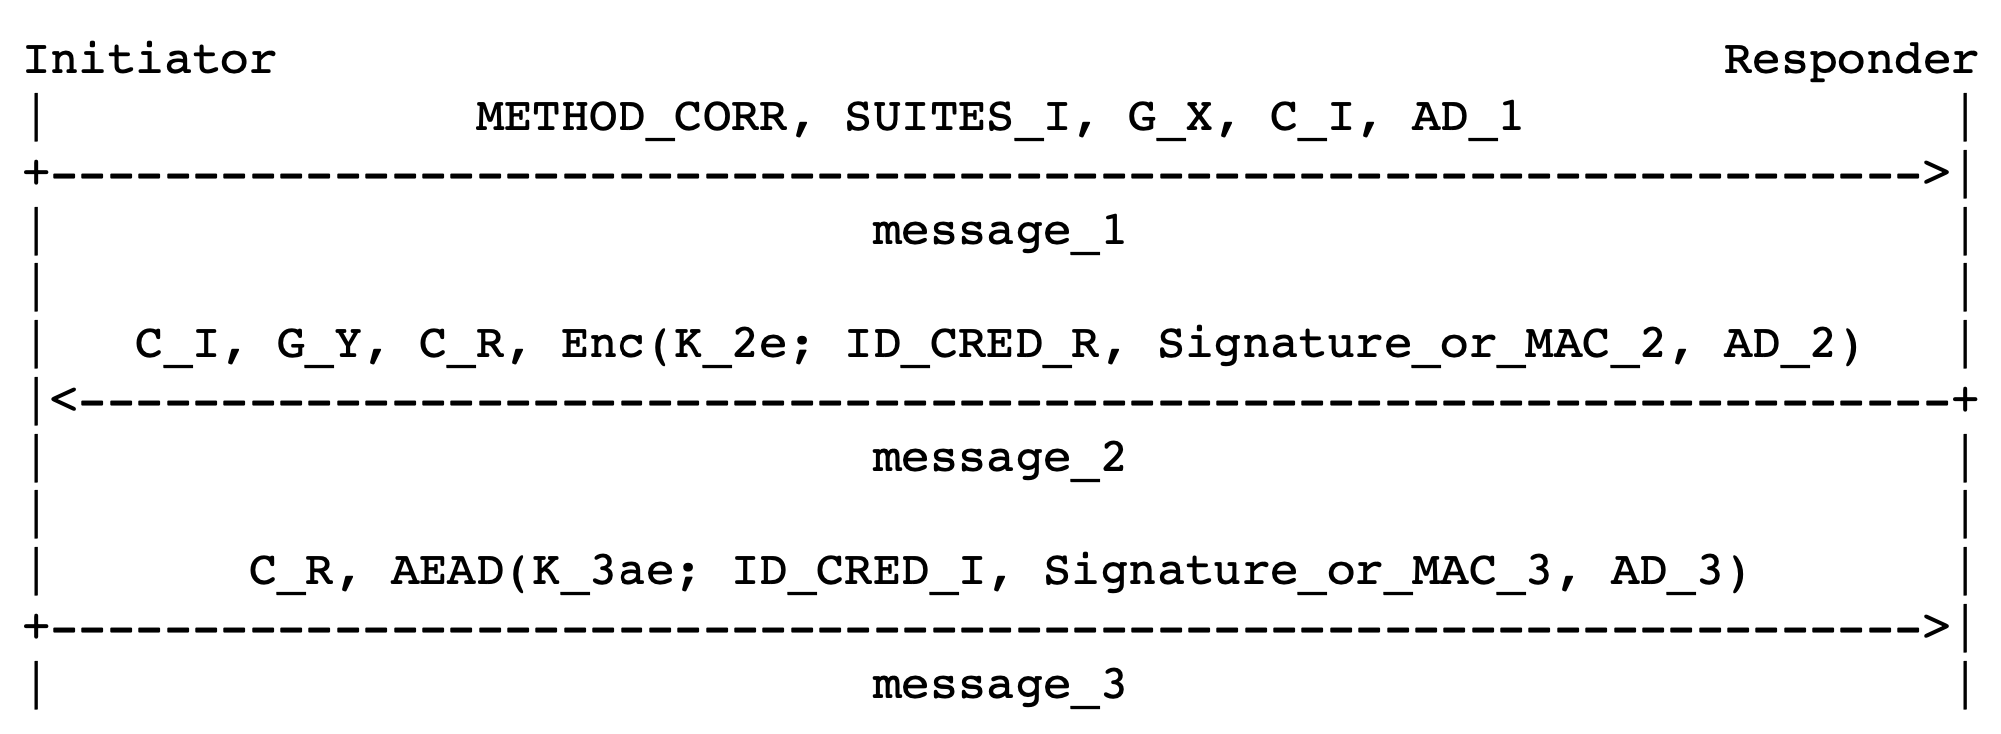
\includegraphics[scale=0.3]{Images/asym.png}
\scalebox{.7}{
\tikzset{>=latex, every msg/.style={draw=thick}, every node/.style={fill=white,text=black}}
\begin{tikzpicture}
    \node (ini) at (0, 0) {Initiator};
    \draw [very thick] (0, -0.5) -- (0,-15.2);
    \draw [very thick] (9, -0.5) -- (9,-15.2);
    \node[below of=ini,fill=white,text=black] {$
    \begin{array}{c}
    \text{Knows}\ $g$,\ \mCredi,\ \mLtki,\ \mIdcredi,\\
    \mCredr,\ \mIdcredr, \mADone,\ \mADthree
    \end{array}
    $};
    \node (res) at (9,0) {Responder};
    \node[below of=res] {$
    \begin{array}{c}
    \text{Knows}\ $g$,\ \mCredr,\ \mLtkr,\ \mIdcredr\\
    \mCredi,\ \mIdcredi, \mADtwo
    \end{array}$};
    \action{5em}{ini}{Generates \mMethod,\ \mSuites,\ \mCi,\ $x$\\$\mGx = g^{x}$};
    \msg{10em}{ini}{res}{\mMsgone: \mMethod, \mSuites, \mGx, \mCi, \mADone};
    \action{11em}{res}{$
      \begin{array}{c}
        \text{Generates } \mCr,\ $y$\\
        \mGy = g^{y}\\
        \mTHtwo = \mHash(\mMsgone, \langle \mCi, \mGy, \mCr \rangle)\\
        \mPRKthree = \mPRKtwo = \mHkdfExtract(\textrm{``\phantom{}''}, g^{xy}) \\
        \mKtwom = \mHkdfExpand(\mPRKthree, \mTHtwo) \\
        \mMactwo = \mAead(\mKtwom; \langle \mIdcredr, \mTHtwo, \mCredr, \mADtwo \rangle; \textrm{``\phantom{}''}) \\
        \mSigtwo = \mSign(\mLtkr; \langle \langle \mIdcredr, \mTHtwo, \mCredr, \mADtwo \rangle, \mMactwo \rangle)\\
        \mKtwoe = \mHkdfExpand(\mPRKtwo, \mTHtwo)
      \end{array}$};
    \msg{25em}{res}{ini}{\mMsgtwo: \mCi, \mGy, \mCr, $\overbrace{\mKtwoe\ \mXor\ \langle \mIdcredr, \mSigtwo, \mADtwo \rangle}^{\mCipher}$};
    \action{26em}{ini}{$
      \begin{array}{c}
        \mPRKthree = \mPRKtwo = \mHkdfExtract(\textrm{``\phantom{}''}, g^{xy}) \\
        \mGiy = \mGy^{\mLtki} \\
        \mPRKfour = \mHkdfExtract(\mPRKthree, \mGiy) \\
        \mTHthree = \mHash(\mTHtwo, \mCipher, \mCr)\\
        \mKthreem = \mHkdfExpand(\mPRKfour, \mTHthree) \\
        \mMacthree = \mAead(\mKthreem; \langle \mIdcredi, \mTHthree, \mCredi, \mADthree \rangle; \textrm{``\phantom{}''}) \\
        \mKthreeae = \mHkdfExpand(\mPRKthree, \mTHtwo) \\
      \end{array}$};
    \msg{37em}{ini}{res}{$\mMsgthree: \mCr, \mAead(\mKthreeae; \mTHthree; \langle \mIdcredi, \mMacthree, \mADthree \rangle$)};
    \action{38em}{res}{$
    \begin{array}{c}
       \mGiy = \mCredi^{y} \\
       \mPRKfour = \mHkdfExtract(\mPRKthree, \mGiy) \\
       \mTHthree = \mHash(\mTHtwo, \mCipher, \mCr)\\
        \mKthreem = \mHkdfExpand(\mPRKfour, \mTHthree) \\
        \mKthreeae = \mHkdfExpand(\mPRKthree, \mTHtwo)
    \end{array}$};
    \draw [line width=2mm] (-2,-15.2) -- (2,-15.2);
    \draw [line width=2mm] (7,-15.2) -- (11,-15.2);
    \end{tikzpicture}}
\caption{The \mStatSig method of \mEdhoc}
\label{fig:edhocstatsig}
\end{figure}

\subsection{\mSigSig method}
In this method, both parties run the \mSig method, and therefore, both the second and third messages need to be signed before being encrypted via \mAead. The pseudorandom string \mPRKtwo is generated as usual, by sending the empty salt and the shared secret to the KDF, and both \mPRKthree and \mPRKfour are set equal to \mPRKtwo. The second message looks like the one from the \mSigStat method described above, while the third looks like the one from the \mStatSig method.

\subsection{Deriving an OSCORE context}
\mEdhoc is often used to set up parameters for \mOscore. In this case, the parties make sure that the connection identifiers are distinct, i.e. $\mCredi \neq \mCredr$, since these are used as \mOscore sender IDs. If the initiator plays the role of the CoAP client, and the responder the role of the CoAP server, the client gets the sender ID \mCredr and the server the ID \mCredi (the identifiers are swapped). The \mAead and hash algorithms for \mOscore stay the same as those used for the selected cipher suite in \mEdhoc, while the master secret for \mOscore is derived using the key length of the \mAead algorithm of \mEdhoc. 

\subsection{Expected security properties}
In this section, we list all the claims made by the authors of~\cite{selander-lake-edhoc-01} regarding the security properties satisfied by \mEdhoc. We will revisit these claims when we discuss the formal modelling and verification of \mEdhoc in the next few sections of the paper. The following are the claims.
\knote{We should link forward to the formalization section where we describe
    exactly what we have verified and what not. We should also link forward to
    the discussion section where we "analyze" these claims from a
    standardization process view point.
}
\vnote{Will do once the formalization section is in.}

\mEdhoc inherits some security properties from the \mSigmaI protocol. These are perfect forward secrecy, mutual authentication with aliveness, consistency, peer awareness (to the responder, but not to the initiator), identity protection, and Key Compromise Impersonation (KCI) resistance.

All methods other than \mPskPsk offer identity protection of the initiator against active attacks and that of the responder against passive attacks. The roles should be assigned to protect the more sensitive identity. This is usually the entity whose identity cannot be inferred from information in the lower layers.

\mEdhoc also provides protection against replay attacks by the attacker. The attacker also cannot affect any negotiated parameters. A single session of \mEdhoc enables the responder to verify that the selected cipher suite is the most preferred of the initiator which is supported by both parties, even though there is no negotiation of cipher suites per se.

In order to reduce the chances of pervasive monitoring, \mEdhoc only supports methods with perfect forward secrecy. One way to limit the effect of breaches is to minimize the use of symmetrical group keys for bootstrapping. \mEdhoc, therefore, uses raw public keys and self-signed certificates instead of symmetrical group keys for bootstrapping.

For the \mPskPsk method, compromising \mPsk lets the attacker impersonate either party in \mEdhoc exchanges with the other. For the other methods, compromising the private authentication keys of one party lets the attacker impersonate only the compromised party in exchanges with other parties. In particular, it does not let the attacker masquerade as any other parties in communications with the compromised party. 

Compromise of the \mHkdf input parameters (ECDH shared secret and/or \mPsk) leads to all session keys derived from that shared secret being deemed compromised. However, the compromise of one session key does not affect other session keys. If the long-term keys (\mPsk or private authentication keys) are compromised, this does not affect the security of instances of \mEdhoc which have completed prior to compromise. 

